\documentclass[10pt,a4paper,oneside]{scrartcl}

% \usepackage[ngerman]{babel} 
\usepackage[USenglish]{babel} % English proposal

\usepackage[utf8]{inputenc}
\usepackage{hyperref,xcolor,microtype,ifthen,csquotes}
\usepackage{graphicx}

\setkomafont{disposition}{}
\setkomafont{descriptionlabel}{\bfseries}

\usepackage[textwidth=450pt]{geometry}

\usepackage[backend=bibtex,style=ieee,hyperref,natbib]{biblatex}

\addbibresource{references.bib}
\addbibresource{BA.bib}


% Disable the hints here
\newboolean{showhints}
\setboolean{showhints}{true}
%\setboolean{showhints}{false}

\newcommand\hint[2]{
\ifthenelse{\boolean{showhints}}{
\begin{center}
\colorbox{black!10}{
\begin{minipage}{.963\textwidth}
#2\hfill\textbf{#1}
\end{minipage}
}\end{center}}{}
}


\newcommand\comment[1]{\textcolor{red}{(#1)}}
% \renewcommand\comment[1]{}

%Title of the proposal
\title{Something Something CouchEdit DSL}
%bachelor or master?
\subtitle{(Bachelor Thesis Proposal)}
%first and then last name
\author{Florian Lappe}

\begin{document}

\maketitle

\section{Introduction and Motivation}
\label{sec:motivation}

% \hint{(this page)}{
% 		An introduction provides readers with the background information for the research proposed (or reported in the paper), with the purpose to provide an understanding of how the research is related to other research \cite{Wilkinson1991}. In an introduction, the writer should \cite{Creswell2008}:
% 		\begin{itemize}
% 		\item Create reader interest in the topic
% 		\item Lay the broad foundation for the problem that leads to the study
% 		\item Place the study within the larger context of the scholarly literature
% 		\item Reach out to a specific audience 
% 		\end{itemize}
% 		}

Modeling languages have long played an important role in software engineering. Well designed models, can abstract complex systems and provide visual aid in understanding them. Furthermore in form of the Business Process Model Notation (BPMN) they are used to define and automate processes. Today, research in the area of Model Driven Engineering (MDE), a paradigm centered around models, with the intent to generate code bases and whole systems from them, the importance of models is rising even more.

As these tasks require syntactic correctness of used models, modeling tools become an essential part of an engineers workflow. Especially visual modeling tools provide -in theory- an intuitive and user friendly way to design models. But, current graphical modeling tools, tend to constraint users in unintuitive ways and deliver sub par user experience (UX). This usually arises from a tight coupling between a modeling tools User interface (UI) and the underlying model. As the models syntax is usually inflexible, the UI has to make amends to adhere to this syntax. this often creates problems for the user like, connections can only be drawn between two existing states, or deleting a node will result in all its children being deleted as well.

To amend these usability woes, L. Nachreiner proposed a novel modeling framework, called CouchEdit \cite{nachreiner_couchedit_2020}. This framework decouples user interface and model syntax by introducing different models for both. Instead of relying directly on the syntax of the model that is being designed, in the CouchEdit architecture, the user interface is using a render model that only consists of nodes that are rendered in the Modeling tool, called concrete syntax. On the other hand, the actual models syntax now stands on its own, called abstract syntax. To translate between concrete and abstract syntax, a syntax meta model is utilized. CouchEdit at its core was designed to be general purpose, meaning it can be rewritten to adhere to any model syntax. But to realize this in the current implementation, the source code has to be rewritten directly, which is error prone, convoluted and requires some understanding of CouchEdits internal architecture.

To create a more developer friendly and flexible way of adapting CouchEdit to different modeling syntaxes, this design research aims to propose a new
domain specific language (DSL), that can be used to configure CouchEdit for
any Modeling syntax. Furthermore a conceptual parser is to be developed and implemented, that provides proof of concept how this newly developed DSL interacts with the CouchEdit architecture.

\section{Problem Statement}
\label{sec:problem_statement}

% \hint{(0,75 pages)}{
% The statement of the problem is the foundation for the construction of any research proposal. In addition to being an integral part of selecting a research topic, it also helps to select research design. It serves as the bases for determining research objectives, formulation of research hypotheses or research questions, and planning the research design \cite{Booth2003}. It allows the researcher to describe the problem systematically, to reflect on its importance, its priority and to point out why the proposed research on the problem should be undertaken. 

% A problem might be defined as the issue that exists in the literature, theory, or practice that leads to a need for the study. It is important in a proposal that the problem stands out and that the reader can easily recognize it. 
% \begin{itemize}
% \item A problem statement should be presented within a context, and that context should be provided and briefly explained, including a discussion of the conceptual or theoretical framework in which it is embedded. 
% \item Clearly and succinctly identify and explain the problem within the framework of the theory or line of inquiry that supports the study. 
% \item State the problem in terms intelligible to someone who is generally sophisticated but who is relatively uninformed in the area of your investigation.
% \end{itemize}

% Effective problem statements answer the question: Why does this research need to be conducted? If the writer is unable to answer this question clearly and succinctly, the statement of the problem will be perceived as vague and diffuse.}      


A general purpose framework should be configurable for multiple use cases in its designated domain. CouchEdit as a general purpose graphical editing framework thus should be configurable for multiple modeling syntaxes. Technically this is possible, as long as one has access to the source code.
But this would mean, every time CouchEdit has to support a new modeling syntax, manual changes in the source code have to be made and the project has to be compiled from sources. The implementation of a DSL parser, that can interpret model syntax definitions at runtime would thus increase flexibility. Furthermore a well designed domain specific language could reduce the amount of knowledge that is needed about the CouchEdit framework.

As a relaxed conformance editing framework, CouchEdit poses special architectural requirements. It has to allow for temporary inconsistencies between concrete syntax (what the user draws) and abstract syntax (what the underlying Model actually looks like). As the concrete syntax does not always have to map to a syntactic correct abstract model, this allows for more freedom in the modeling process (e.g. dangling transitions).

CouchEdit achieves this by building upon the architecture concept of clear separation between concrete and abstract syntax, proposed by Y. Van Tendeloo et al. \cite{van_tendeloo_concrete_2017}. Internally, CouchEdit builds a hypergraph, that maps the given concrete syntax to all possible abstract syntaxes (interpretation of a concrete syntax can be ambiguous and thus multiple abstract syntaxes can be possible). To build this Hypergraph, a set of Processors is employed, which are connected in a reactive publish and subscribe pattern. All Processors -and the user interface- are subscribed to a bus (fig. \ref{fig:processors}). If a change (diff) is published to the bus (e.g. the user adds a node to the concrete syntax), all processors that are subscribed to this type of diff are notified and calculate new resulting diffs, these new diff are then also published to the bus and all processors interested in these new diffs are invoked as well.

\begin{figure}
  \label{fig:processors}
  \centering
  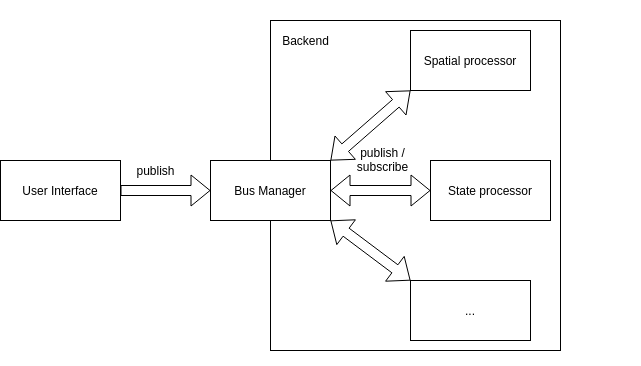
\includegraphics[width=.6\linewidth]{./couchedit-processors}
  \caption{Publish Subscribe architecture of CouchEdit}
\end{figure}

Some of these processors are needed for every type of syntax model, for example the spatial processor, that processes how nodes in the concrete syntax are positioned to each other (above, besides, etc.). Other processors are specific to the given modeling syntax, for example a state chart syntax would require a state processor, that processes if a given graphical object represents a state (usually true if the given node is a rectangle with rounded edges).

A modeling syntax parser for CouchEdit would have to generate these syntax specific processors. while considering multiple design constraints that result from this architecture. Thus a DSL is needed that defines the desired abstract modeling syntax and specifies how a concrete graphical syntax can be mapped to this abstract syntax. While there is ongoing research in the area of relaxed conformance editing and how to link concrete and abstract syntax, it does not immediately become clear what such a domain specific language would look like.


% \begin{itemize}
%   \item The undirected publish/subscribe pattern allows for the generation of a set of processors that publish diffs to trigger each other which would result in an endless processing loop. 
%   \item the generated processors should be decoupled as much as possible, as this allows for better parallelization.
%   \item The order in which diffs are published can not influence the resulting hypergraph.
%   \item Processors should be triggered on as few diff types as possible, to reduce the amount of pattern recognition that has to be done.
% \end{itemize}





% As the cornerstone this research builds upon, CouchEdit is of great significance. CouchEdit falls under the category of relaxed conformance editing, meaning, it allows for temporary inconsistencies between concrete syntax (what the user draws) and abstract syntax (what the underlying Model actually looks like). As the concrete syntax does not always have to map to a syntactic correct abstract model, it allows for more freedom in the modeling process, for example, dangling transitions. 

% CouchEdit realizes this by building upon the architecture concept of clear separation between concrete and abstract syntax, proposed by Y. Van Tendeloo et al. \cite{van_tendeloo_concrete_2017}. Internally, CouchEdit builds a hypergraph, that maps the given concrete syntax to all possible abstract syntaxes (interpretation of a concrete syntax can be ambiguous and thus multiple abstract syntaxes can be possible). To build this Hypergraph, a set of Processors is employed, which are connected in a reactive publish and subscribe pattern. All Processors -and the user interface- are subscribed to a bus (fig. \ref{fig:processors}). If a change is published to the bus (e.g. the user adds a node to the concrete syntax), all processors that are subscribed to this type of change are notified and calculate new resulting changes, these new changes are then also published to the bus and all processors interested in these new changes are invoked. 



% Some of these processors are needed for every type of syntax model, for example the spatial processor, that processes how nodes in the concrete syntax are positioned to each other (above, besides, etc.). Other processors are specific to the given Syntax model, for example the state processor for a state chart syntax, that processes if a given node represents a state (usually true if the given node is a rectangle with rounded edges). The DSL parser that is part of the proposed design research would need to generate syntax specific processors from the DSL.


\section{Purpose of the study}

% \hint{(0,25 pages)}{The purpose statement should provide a specific and accurate summary of the overall purpose of the study. Briefly define and delimit the specific area of the research. Incorporate the rationale for the study. A commonly used sentence starts with: ''The purpose of this study is \ldots''. The purpose should clarify who is anticipated to benefit from the results of your study and how the results may be used.}

The purpose of this study is to develop a domain specific language, for the CouchEdit Framework. This DSL is supposed to provide a comprehensive and easy to use way for defining new modeling languages. Furthermore a prototypical parser is to be implemented, that can comprehend this newly designed DSL and translate it into a set of CouchEdit processors.

This extension of the CouchEdit framework is supposed to improve developer accessibility and framework flexibility, as the implementation of an external DSL and its corresponding parser means that the system does not have to be recompiled from source code every time a different modeling syntax is to be used. Furthermore in the current implementation, to support new modeling syntax, the user is forced to write processors on source code level, which is convoluted and requires understanding of most of the CouchEdit architecture. By designing a comprehensible DSL syntax, users will have an easier time defining new modeling syntax.



\section{Review of the literature}

% \hint{(1 page)}{
%   The literature review provides the background and context for the research problem. It should establish the need for the research and indicate that the writer is knowledgeable about the area. The literature review:
%   \begin{itemize}
%     \item Describes the results of other studies that are closely related to the study being proposed (or reported)
%     \item Relates a study to the larger, ongoing dialogue in the literature about a topic, filling in gaps and extending prior studies
%     \item Provides a framework for establishing the importance of the study, as well as a benchmark for comparing the results of a study with other findings
%     \item “Frames” the problem earlier identified
%   \end{itemize}
%   The literature review should demonstrate to the reader that you have a comprehensive grasp of the field and are aware of important recent substantive and methodological developments. Define the starting point for your study - how will your study refine, revise, or extend what is now known?

%   In a proposal, the literature review is generally brief and to the point. Select and reference only the more appropriate citations. Make key points clearly and succinctly. Later in your thesis, you will elaborate on this section.


%   Initial literature related to the specific topic. This will be a small selection of papers relevant to the work, agreed on with the supervisor. The purpose of this section is to demonstrate problems or limitations of existing solutions.}


% The DiaGen project \cite{minas_concepts_2002}, similar to CouchEdit strives to provide a form of relaxed conformance visual editing. It provides a toolkit for generation of diagram editors. In its initial stages it consisted of a java library that contains the necessary parts of a functioning diagram editor, as well as a generator that can generate Java code from a given given specification file that uses a custom DSL developed for the DiaGen project. The toolkit was later extended by a designer application that provides a more intuitive way of defining the editor specification. Furthermore EMF support was added for generation of the Model syntax.


\begin{description}
  \item[CouchEdit - a modular graphical editing architecture for flexible modeling] \cite{nachreiner_couchedit_2020}

        \begin{description}
          \item[Authors:] L. Nachreiner
          \item[Summary:] In this work, the CouchEdit architecture is first proposed, an initial prototype is developed and the results are evaluated.
          \item[Significance:] As CouchEdit builds the foundation of the proposed research, this work lays out most of the constrains and rules that the designed DSL has to adhere to. A thorough analysis of CouchEdits features and architecture will be integral to a successful DSL design. Furthermore the developed prototype will be used as the base for the DSL parser implementation.

        \end{description}

  \item[Specifying and Implementing Visual Process Modeling Languages with DiaGen] \cite{minas_specifying_2001}
        \begin{description}
          \item[Authors:] M. Minas, B. Hoffmann
          \item[Summary:] DiaGen is a tool for automatic generation of visual modeling editors\footnote{DiaGen: \url{http://www2.cs.unibw.de/tools/DiaGen}}. A DSL is used to define properties of the editor as well as specification of how to process the model syntax. DiaGen builds a hypergraph structure from the model that is drawn in the editor. With the help of reduction rules and grammar definitions, this hypergraph is then transformed into an abstract syntax representation of the defined modeling language.
          \item[Significance:]  DiaGen implements a domain specific language for transformation from concrete render syntax to abstract model syntax and thus provides a potential baseline that could be used in a similar DSL definition for the CouchEdit framework.
          \item[Delimitations:] DiaGens DSL is used to generate java source code, which then can be compiled into a working editor. This means that the DSL generator has some leniency as potential flaws can be adjusted in the code itself. As this research strives to develop an implementation that parses at runtime, the same leniency can not be applied. On the other hand, DiaGen generates a fully functioning editor and thus has to generate implementations of UI components. CouchEdit intends to be Editor agnostic and therefore only has to provide a definition of graphical objects that are used in the configured modeling syntax.

        \end{description}

  \item[Making Metamodels Aware of Concrete Syntax] \cite{hutchison_making_2005}
        \begin{description}
          \item[Authors:] F. Fondement, T. Baar
          \item[Summary:] The Authors propose an approach to the interpretation of concrete syntax. A set of graphical objects is summarized into a display class which is then mapped to a so called display manager which itself is mapped to an abstract syntax object. This display manager has the job of keeping display class an abstract syntax object in sync. For this to be possible, constraint rules are defined for display managers using the Object Constraint Language (OCL).
          \item[Significance:] Similar to CouchEdit, the proposed concept works with a clear separation of concrete and abstract syntax. The approach of using OCL rules to keep abstract and concrete syntax in sync could potentially applied to a CouchEdit DSL, as the internal diff based system often has to apply similar transformations.
          \item[Delimitation:] the proposed design is wrapping graphical objects in display classes and thus can map one abstract object to exactly one Display object. In its current implementation CouchEdit in many cases maps one Abstract object to multiple graphical objects, which could limit the applicability of this work. It would have to be evaluated if the Display class grouping mechanism can be incorporated into the CouchEdit Framework, but as implementation of that functionality was left open it is unclear how it would actually have to be defined.
        \end{description}

  \item[Correctly defined concrete syntax] \cite{baar_correctly_2008}
        \begin{description}
          \item[Authors:] T. Baar
          \item[Summary:] The author proposes a way to formally define a models concrete syntax and how to link it to the abstract syntax. Similar to \cite{hutchison_making_2005}, they use display managers that are defined using OCL. Furthermore an algorithm is given to check a concrete syntaxes correctness.
          \item[Significance:] This work gives additional insight on using OCL as a language to define concrete syntax mappings. Furthermore it provides hints to what is needed for checking syntax correctness. While implementing syntax correctness checking is beyond the proposed researches scope, it will still be worthy to keep this in mind when designing a DSL applicable to CouchEdit.
        \end{description}


\end{description}

\section{Research questions and/or Hypotheses}
\label{sub:questions}

% \hint{(0,25 Pages)}{
%   Questions are relevant to descriptive, normative or census type research. (What are relevant factors? How many of them are there? Is there a relationship between them?) Hypotheses are relevant to theoretical research, and when you state hypotheses the reader is entitled to have an exposition of the theory that lead to them (and the assumptions underlying the theory).

%   In general, you should be prepared to interpret any possible outcome with respect to the questions or hypotheses. Try to visualize in your mind tables or other summary devices, which you expect to come out of the research, short of the actual data.


%   Research questions describe one or several main questions of the thesis, as well as several subquestions agreed upon with the supervisor. Research questions can be split in several types and are typically W-questions (why, what, how, \dots).\footnote{based on \url{http://www.studieren.at/uni-abc/forschungsfrage-welche-fragetypen-gibt-es} (German).}
%   %
%   \begin{description}
%     \item[Explanation:] Why is something the way it is?
%     \item[Description:] What do different approaches look like?
%     \item[Prediction:] How will something develop?
%     \item[Assessment:] How can the described/explained be assessed?
%   \end{description}

%   These questions should be written such that they can be answered within the thesis, and they should fully cover the research problem.
% }

The primary goal of this research will be the development of a domain specific language for the CouchEdit framework. This imposes multiple questions which are to be answered in order to design and evaluate the designated DSL.

\begin{description}
  \item[RQ1:] Is it possible to define a concise domain specific Language that covers CouchEdits complete feature set?

        If this is not possible, the following question has to be answered.
        \begin{description}
          \item[RQ1.1:] How could the feature set be narrowed down, without impacting the frameworks capabilities to much?
        \end{description}

  \item[RQ2:] What requirements does the CouchEdit architecture impose onto a domain specific language?

        The architectures characteristics and quirks have to be considered when designing the language. For example, the publish and subscribe pattern, that is used, could make it easy to introduce nonterminating processing chains, which the DSL should hinder where possible.

  \item[RQ3:] Could an automatic generation of CouchEdit processors, impact the frameworks performance?

        Control over the implementation specifics is gated by the DSL interface which reduces optimization potential and thus could introduce performance issues in some cases.
\end{description}

\section{The Design - Methods and Procedures}
\label{sec:approach}

% \hint{(0,5 Pages)}{
%   Any research or problem solving requires a systematic approach with methods and procedures. Indicate the steps you will take to answer every question or to test every hypothesis indicated in the previous section, to solve the problem that you are addressing. There are several research methods, e.g. design research \cite{Collins2004,Vaishnavi2004,Oesterle2011}, case study \cite{Runeson2008, Yin2009}, action research \cite{McKay2001}, Survey \cite{Malhotra1998}, and experiment \cite{Basili1986} just to mention a few. Different research methods and procedures require different descriptions.

%   For example for a survey, it becomes vital to describe sampling and instrumentation. The sampling, i.e. the population and how the sample has been drawn from that, needs to be described to clarify to what extent the findings of a study can be generalized to people or situations. You should also outline the instruments you propose to use (surveys, scales, interview protocols, observation grids). For a case study or a design research, other aspects become vital.

%   \textit{Data collection}
%   For all studies, you need to have a systematic approach for data collection. Outline the general plan for what data to collect, and how. This may include survey administration procedures, interview or observation procedures. Also, provide a general outline of the time schedule you expect to follow.

%   \textit{Data Analysis}
%   For all studies, you need to have a systematic approach for data analysis. Specify the procedures you will use to analyze your data. If coding procedures are to be used, describe these in reasonable detail. For evaluations, describe the criteria to be used in reasonable detail.


%   Describe the initial ideas for the thesis and the first steps to answer the research questions. Ideas can be pointers towards promising ideas in the literature (not necessarily read completely) or some sketch of how ideas from the literature may be developed. It does not need to be a concrete idea, but should indicate what will be done in the first weeks after the proposal is done.}



As this research strives to develop a new domain specific language suitable for the CouchEdit framework, it will be conducted in accordance to the Design Science Research (DSR) approach. According to V. Vaishnavi et al. a design science research process consists of five steps\cite{Vaishnavi2004}.

\subsection{Problem Awareness}
The first step of a design science research is the identification of existing problems. As specified in section \ref{sec:problem_statement}, it was identified that the current CouchEdit implementation lacks an user friendly way of adapting it to different modeling syntaxes and that it is unclear how a DSL for this architecture would look like.

\subsection{Suggestion}
With a clear definition of the problem, objectives can be proposed which have to be achieved in order to solve this problem. The first objective of this research is to develop a DSL for the CouchEdit architecture. To be more precise, a DSL is to be designed, that can be used to specify syntax metamodel definitions which map concrete graphical syntaxes to Abstract syntax models, and is applicable to CouchEdits architecture. The second objective is to implement a prototype that provides proof of concept, for the applicability of the design DSL.


\subsection{Development}
The primary goal of a design science research is the development of artifacts.
The first artifact to be developed in this research will be a domain specific language, that can be used to define new modeling syntaxes for a relaxed conformance editor and is applicable to CouchEdits architecture. The second artifact that is to be developed, is a parser prototype that can translate the developed DSL into a CouchEdit implementation which will be able to process, the defined modeling syntax.

To this end, the first sub step of the development stage will be to do a comprehensive analysis of CouchEdits architecture. In his work L. Nachreiner describes in detail, which modeling features his framework covers and how they are implemented \cite{nachreiner_couchedit_2020}. For each of these features it has to be checked if they can be represented by the approaches of \cite{minas_specifying_2001} and \cite{hutchison_making_2005} in a concise way (RQ1). Should this not be possible for all features, it would have to be checked if these approaches can be extended. if this is not possible as well, it would have to be seen if the problematic features could be dropped or simplified to allow for a concise syntax definition (RQ1.1).

this process should result in the basic version of an applicable DSL. in the next sub step, the parser will be implemented, this is an iterative step. first, a parser implementation will be developed on the basis of the designed DSL, this should reveal further requirements imposed by CouchEdits architecture (RQ2). The DSL then has to be adjusted to account for these requirements, which in turn requires changes of the parser until no further requirements can be deduced. 

\subsection{Evaluation}
Now that desired artifacts are fully developed it has to be evaluated how well they do their designated task. the artifacts can be evaluated by means of feature completeness as well as performance. L. Nachreiner wrote extensive test cases for his manual implementation of a sub set of the state chart language. his test cases and performance results can be used to evaluate the developed artifacts (RQ3). This should highlight potential flaws of the designed artifacts, which can be addressed -if time allows- by going back to the development stage and revising the artifacts.
\subsection{Conclusion}
The conclusion stage marks the end of a DSR and the results are written up. This works written part will be the resulting bachelor's thesis as well as all source code and documentation.



\section{Limitations and Delimitations}
% \hint{(0,5 pages)}{
%   A limitation identifies potential weaknesses of the study. Think about your analysis, the nature of self-report, your instruments, and the sample. Think about threats to external or internal validity that may have been impossible to avoid or minimize and explain these.

%   Delimitation addresses how a study will be narrowed in scope. This is where you explain the things that you are not doing and why you have chosen not to do them. For example, the literature you will not review (and why not), the population you are not studying (and why not), the methodological procedures you will not use (and why not). Limit your delimitations to the things that a reader might reasonably expect you to do (given your topic and problem statement) but that you, for clearly explained reasons, have decided not to do.}

As this research has tight time constraints some topics have to be left out. For once, while concrete syntax correctness checking is an important part of a complete implementation, it would require to much extra time. Furthermore, static syntax analysis by the DSL parser would probably improve developer experience but is out of scope as well. Lastly, while evaluating the DSLs usability would be desirable to validate the DSLs advantages, this would require a survey, which also falls completely beyond this works time constraints.

\section{Significance of the study}
% \hint{(0,25 pages)}{Indicate how your research will refine, revise, or extend existing knowledge in the area under investigation. Note that such refinements, revisions, or extensions may have substantive, theoretical, or methodological significance. Think pragmatically.

%   Most studies have two potential audiences: practitioners and researchers. Think about implications: What implications may the results of the study have on research? What implications may the results of the study have on practice? }

This work will extend and combine existing research in the field of syntax meta modeling. While many works formalize concrete syntax definition and a mapping to an existing abstract syntax, only few actually provided a working implementation.

This work will produce new information on how to use syntax meta modeling to define modeling languages for relaxed conformance editing frameworks.


\section{Planning}
\label{sec:planning}

\subsection{Own Background}
\label{sub:background}

% \hint{(0,25 Pages)}{Relevant background on methodologies and tools (e.g., process models, appropriate formal models, formal specifications languages, algorithms) from lectures, seminars and jobs. Also write down the necessary skills that need to be learned during the thesis.}

I bring general experience in software engineering from previous projects in university and as a student assistant. I have prior experience with Kotlin, JavaFX and reactiveX, as well as dependency injection, which will be beneficial during the implementation phase. The most important new skill to acquire will be an understanding of DSL development as no prior experience is present. Furthermore knowledge about language parsers such as Xtext or ANTLR, as well as some understanding of GMF will be required for the implementation phase.



\subsection{Work packages}
\label{sub:wp}

% \hint{(0,25 Pages)}{General description of the work that needs to be done per month. The time plan should be consistent with the research questions (\ref{sub:questions}) and the necessary background (\ref{sub:background}) and potential wait time for resource.}

\begin{description}
  \item[W1-2:] Learning basics
        \begin{itemize}
          \item Read into DSL design
          \item Learn to create DSL parsers with xtext/ANTLR
          \item How to generate abstract syntax models
        \end{itemize}
  \item[W3-4:] Design
        \begin{itemize}
          \item Compare CouchEdit features against existing approaches
          \item Design fitting DSL on the basis of this.
        \end{itemize}
  \item[W5-6:] Implementation
        \begin{itemize}
          \item Develop Kotlin internal DSL to create processors
          \item Implement external DSL parser
          \item Change existing UI to use DSL concrete syntax definitions
        \end{itemize}
  \item[W7-8:] Evaluation
        \begin{itemize}
          \item Adapt existing test cases to the developed parser
          \item Performance comparison
          \item Potential improvements
        \end{itemize}
  \item[W9-12:] Write thesis
\end{description}

\subsection{Contingency plan}
\label{sub:contingency}

% \hint{(0,5 Pages)}{Possible risks (e.g., no available resources) that can already be estimated before starting the thesis, as well as possible contingency plans.}

\begin{enumerate}
  \item \textbf{Risk} CouchEdit architecture to complex

        \textbf{Contingency} If it is determined that CouchEdits features can't be satisfied using the existing approaches. It would have to be seen if the existing approaches can be extended or else some features could be cut out. Otherwise a new approach would be needed which would completely go beyond the defined time limit. 

  \item \textbf{Risk} Performance problems of implementation

        \textbf{Contingency} The developed parser could introduce performance issues. If possible, the parser implementation could be optimized, else the limiting DSLs capabilities could increase performance or help to limit the possibilities of developers designing definitions that would result in bottlenecks.
\end{enumerate}

\nocite{*}
\printbibliography

\end{document}

